\documentclass[a4paper]{article} 
\addtolength{\hoffset}{-2.25cm}
\addtolength{\textwidth}{4.5cm}
\addtolength{\voffset}{-3.25cm}
\addtolength{\textheight}{5cm}
\setlength{\parskip}{0pt}
\setlength{\parindent}{0in}

%----------------------------------------------------------------------------------------
%	PACKAGES AND OTHER DOCUMENT CONFIGURATIONS
%----------------------------------------------------------------------------------------
\usepackage{bm} % Bold math symbols, !must be loaded before unicode-math!
\usepackage{blindtext} % Package to generate dummy text
\usepackage{enumerate} % Enumerate with redefinable labels
\usepackage{enumitem} % Enumerate with redefinable labels
\renewcommand{\thesubsection}{\thesection.\alph{subsection}} % Enumerate subsections with letters
\renewcommand{\thesubsubsection}{\thesubsection.\roman{subsubsection}} % Enumerate subsubsections with roman numerals
\usepackage{charter} % Use the Charter font
\usepackage[utf8]{inputenc} % Use UTF-8 encoding
\usepackage{microtype} % Slightly tweak font spacing for aesthetics
\usepackage[english, ngerman]{babel} % Language hyphenation and typographical rules
\usepackage{amsthm, amsmath, amssymb} % Mathematical typesetting
\newcommand{\argmax}[1]{\underset{#1}{\text{arg max}}\;}
\newcommand{\argmin}[1]{\underset{#1}{\text{arg min}}\;}
\newcommand{\mb}[1]{\mathbf{#1}}  % Bold math symbols shorthand
\usepackage{float} % Improved interface for floating objects
\usepackage[final, colorlinks = true, 
            linkcolor = black, 
            citecolor = black]{hyperref} % For hyperlinks in the PDF
\usepackage{graphicx, multicol} % Enhanced support for graphics
\usepackage{xcolor} % Driver-independent color extensions
\usepackage{marvosym, wasysym} % More symbols
\usepackage{rotating} % Rotation tools
\usepackage{censor} % Facilities for controlling restricted text
\usepackage{listings, style/lstlisting} % Environment for non-formatted code, !uses style file!
\usepackage{pseudocode} % Environment for specifying algorithms in a natural way
\usepackage{style/avm} % Environment for f-structures, !uses style file!
\usepackage{booktabs} % Enhances quality of tables
\usepackage{tikz-qtree} % Easy tree drawing tool
\usepackage{todonotes} % Tool to insert TODOs
\tikzset{every tree node/.style={align=center,anchor=north},
         level distance=2cm} % Configuration for q-trees
\usepackage{style/btree} % Configuration for b-trees and b+-trees, !uses style file!
\usepackage[backend=biber,style=numeric,
            sorting=nyt]{biblatex} % Complete reimplementation of bibliographic facilities
% \addbibresource{ecl.bib}
\usepackage{csquotes} % Context sensitive quotation facilities
\usepackage[yyyymmdd]{datetime} % Uses YEAR-MONTH-DAY format for dates
\renewcommand{\dateseparator}{-} % Sets dateseparator to '-'
\usepackage{fancyhdr} % Headers and footers
\pagestyle{fancy} % All pages have headers and footers
\fancyhead{}\renewcommand{\headrulewidth}{0pt} % Blank out the default header
\fancyfoot[L]{} % Custom footer text
\fancyfoot[C]{} % Custom footer text
\fancyfoot[R]{\thepage} % Custom footer text
\newcommand{\note}[1]{\marginpar{\scriptsize \textcolor{red}{#1}}} % Enables comments in red on margin
\newcommand{\iverson}[1]{\ensuremath{[#1]}} % Enables Iverson brackets
%----------------------------------------------------------------------------------------

\begin{document}

%-------------------------------
%	TITLE SECTION
%-------------------------------

\fancyhead[C]{}
\hrule \medskip % Upper rule
\begin{minipage}{0.295\linewidth} 
\raggedright
\footnotesize
Ryan Ott \hfill\\   
14862565 \hfill\\
ryan.ott@student.uva.nl
\end{minipage}
\begin{minipage}{0.4\linewidth} 
\centering 
\large 
Practical Assignment 2\\ 
\normalsize 
Deep Learning 1\\ 
\end{minipage}
\begin{minipage}{0.295\linewidth} 
\raggedleft
\today\hfill\\
\end{minipage}
\medskip\hrule 
\bigskip

%-------------------------------
%	CONTENTS
%-------------------------------

\section{Transfer Learning}
\subsection{Comparing Models}
\subsubsection{Inference Speed per Image against Accuracy and Number of Parameters}
With a Pearson correlation coefficient of 0.85 there seems to be a strong positive linear correlation between the
top-1 accuracy and the inference speed. The ViT-B/32 model performs best overall with a higher accuracy for its
inference speed than the trend suggests. Shown in Figure \ref{fig:Top1Acc-vs-Inference}.
\begin{figure}[h]
    \centering
    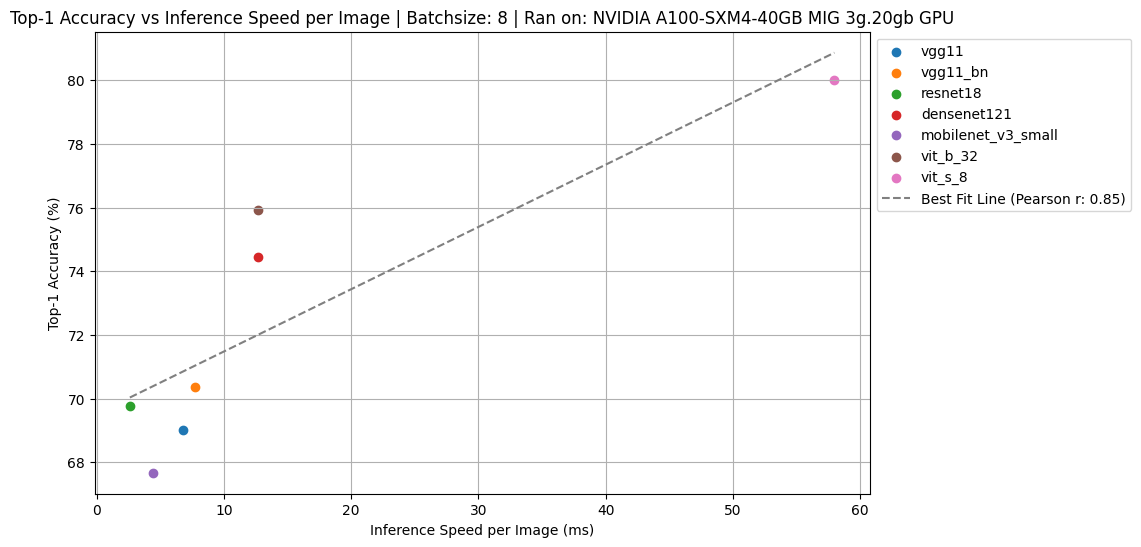
\includegraphics[width=0.75\linewidth]{"imgs/Top1Acc-vs-Inference.png"}
    \caption{Top-1 Accuracy vs Inference Speed per Image}
    \label{fig:Top1Acc-vs-Inference}
\end{figure}

For inference speed against number of trainable parameters, we see no correlation. The number of trainable parameters
should only play a role when the model is being trained, not during inferencing, so this result matches our
expectations. Shown in Figure \ref{fig:NumParams-vs-Inference}.
\begin{figure}[h]
    \centering
    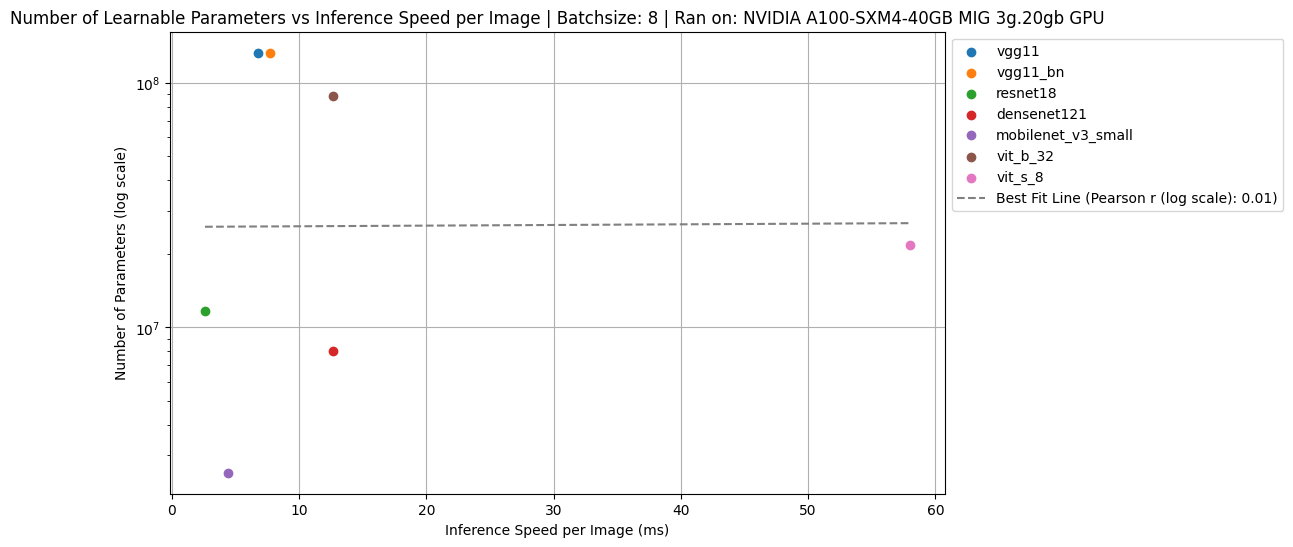
\includegraphics[width=0.75\linewidth]{"imgs/NumParams-vs-Inference.png"}
    \caption{Number of Trainable Parameters vs Inference Speed per Image}
    \label{fig:NumParams-vs-Inference}
\end{figure}

\subsubsection{Inference Speed per Image with and without torch.no\_grad()}
With torch.no\_grad() the inference speed should be faster because gradients are not computed and stored for the
backward pass within the context manager's scope, thus requiring less operations and saving compute. This is
confirmed by the results, the inference speed is slightly faster with torch.no\_grad() across the models. Shown in
Figure \ref{fig:Inference-vs-noGrad}.
\begin{figure}[h]
    \centering
    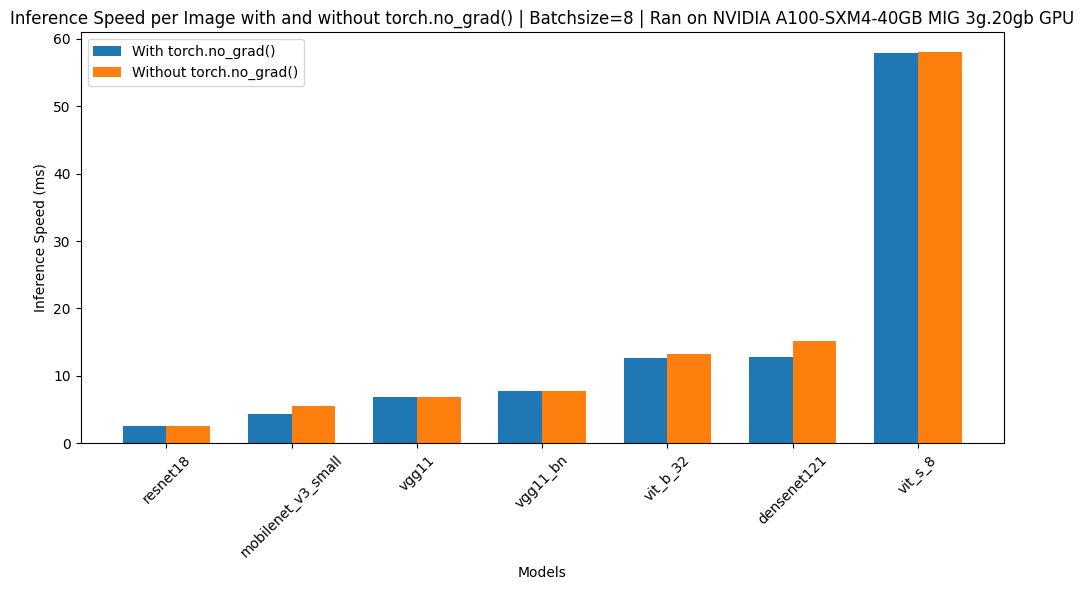
\includegraphics[width=0.75\linewidth]{"imgs/Inference-vs-noGrad.png"}
    \caption{Inference Speed per Image with and without torch.no\_grad()}
    \label{fig:Inference-vs-noGrad}
\end{figure}

\subsubsection{vRAM Usage with and without torch.no\_grad()}
Like with the inference speed, the vRAM usage should be lower with torch.no\_grad() because gradients are not
stored for the backward pass when performing tensor operations, freeing up memory. Much more considerably than the
inference speed, the vRAM usage is lower when using torch.no\_grad() as seen in the plot. Shown in Figure
\ref{fig:VRAM-vs-noGrad}.
\begin{figure}[h]
    \centering
    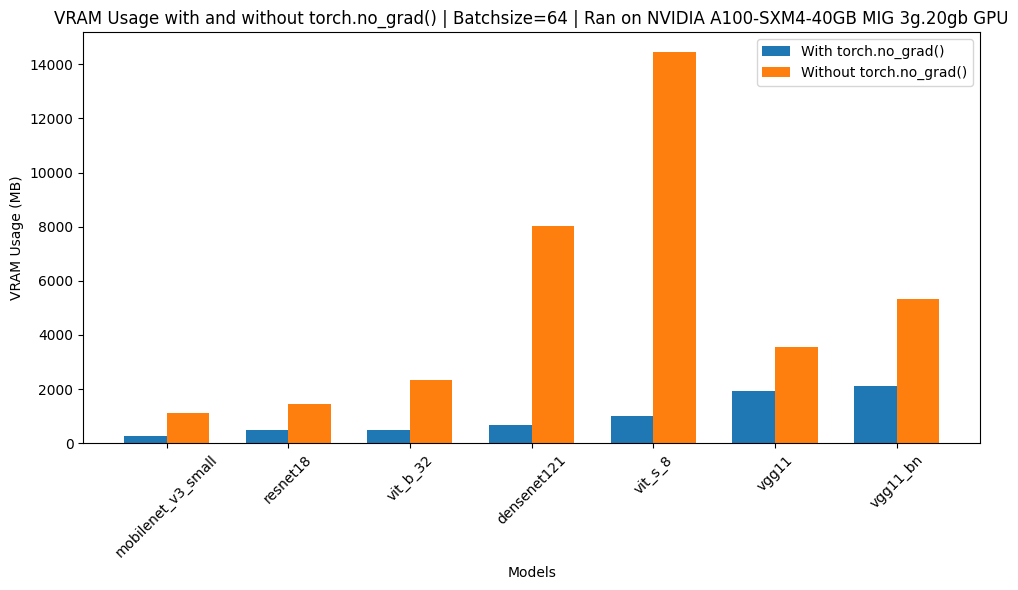
\includegraphics[width=0.75\linewidth]{"imgs/VRAM-vs-noGrad.png"}
    \caption{vRAM Usage with and without torch.no\_grad()}
    \label{fig:VRAM-vs-noGrad}
\end{figure}
\bigskip
% ------------------------------

\subsection{Fine-tuning}
\subsubsection{Retraining ResNet-18's Fully Connected Layer}
Using the specifications and default hyperparameters from the assignment, the retrained model achieved a test
accuracy of 58.55\% in CIFAR-100.

\subsubsection{Increasing Model Performance using Data Augmentation}
By applying \texttt{torchvision.transforms.RandomHorizontalFlip(p=0.5)} around half of the images in the training
set are flipped horizontally. This should increase the model's performance because it is being trained on more
varied data, thus making it more robust to different inputs. The model achieved a test accuracy of 59.27\%, a small
improvement.

\subsubsection{Last vs First Convolutional Layer}
The first convolutional layers tend to capture lower-level features like edges, corners or textures, while the last
layers capture higher-level features like shapes and objects in a larger receptive field. As such, better performance
should be achievable by fine-tuning the last layers (along with the classifier layers) because they are more
specialized to the downstream task than the first layers.
\bigskip
% ==============================

\section{Visual Prompting}
\subsection{CLIP Baseline}
\subsubsection{Top-1 Accuracy on CIFAR-10 and CIFAR-100 with CLIP ViT-B/32 Backbone}
% Zero-shot CLIP top-1 accuracy on cifar10/train: 88.726
% Zero-shot CLIP top-1 accuracy on cifar10/test: 88.94
% Zero-shot CLIP top-1 accuracy on cifar100/train: 63.564
% Zero-shot CLIP top-1 accuracy on cifar100/test: 63.14999999999999
\begin{table}[h]
    \centering
    \begin{tabular}{|l|c|c|}
    \hline
    \rowcolor{Gray}
    \textbf{Dataset} & \textbf{Train Accuracy (\%)} & \textbf{Test Accuracy (\%)} \\ \hline
    CIFAR-10 & 88.73 & 88.94 \\ \hline
    CIFAR-100 & 63.56 & 63.15 \\ \hline
    \end{tabular}
    \caption{Zero-shot CLIP Top-1 Accuracy on CIFAR-10 and CIFAR-100}
    \label{tab:clip_accuracy}
\end{table}


\subsubsection{Prompting CLIP for a New Classification Task}
\textbf{Prompt:} \textit{"This is an image mostly coloured \_\_\_"}\newline
\textbf{Labels:} \textit{"red", "green", "blue"}
\begin{figure}[h]
    \centering
    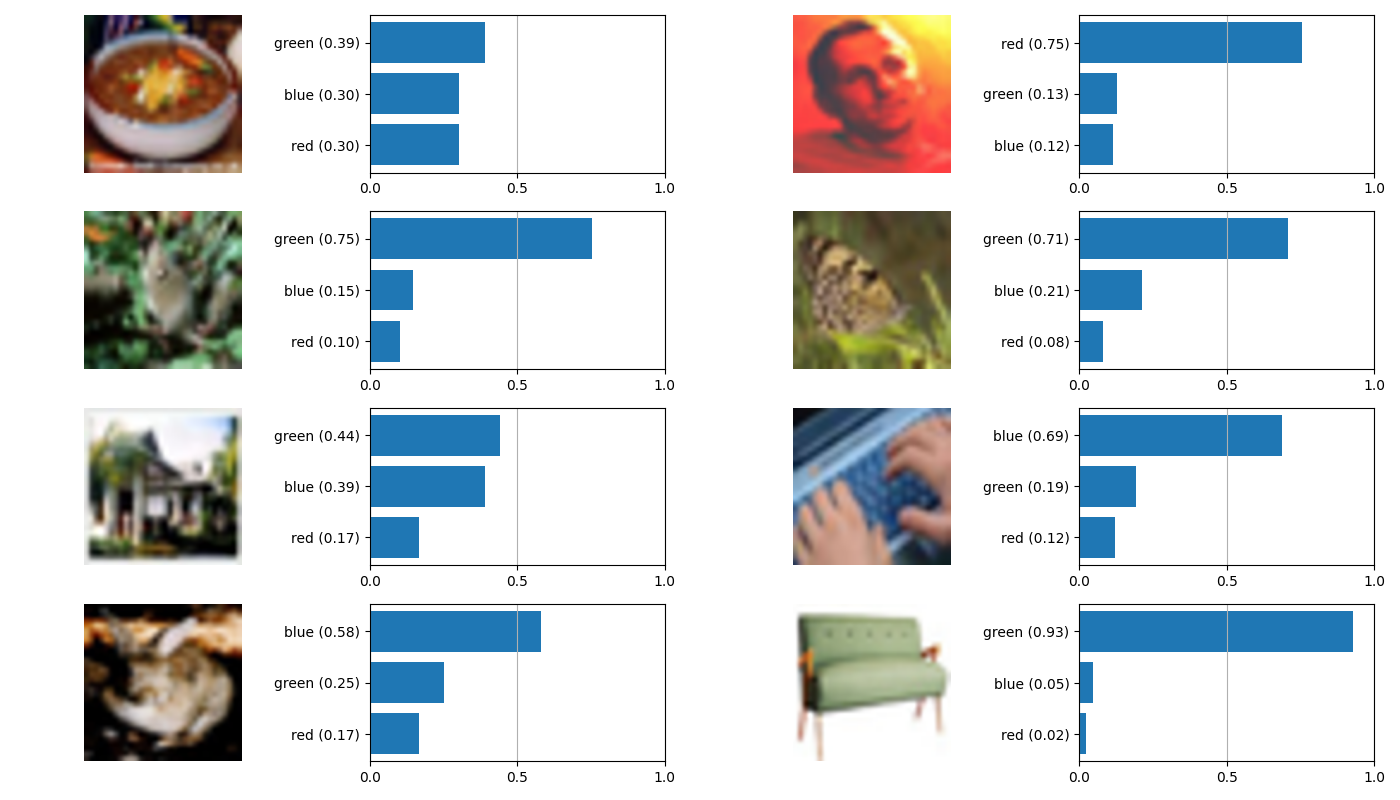
\includegraphics[width=0.75\linewidth]{"imgs/cifar100-test_red,green,blue.png"}
    \caption{Primary Colour Identification}
    \label{fig:CLIP-primary-colour}
\end{figure}

We see in Figure \ref{fig:CLIP-primary-colour} that the model is able to identify the primary colour of the image
with a high degree of accuracy. For images with a distinct primary colour, the model is able to identify it with
high confidence, and for images with no clear distinct primary colour, it returns failry spread out probabilities.
The contrastive learning approach of CLIP allows it to generalize well to new tasks using prompting.
\bigskip

\textbf{Prompt:} \textit{"This image displays an object that is \_\_\_"}\newline
\textbf{Labels:} \textit{"human-made", "from-nature"}
\begin{figure}[h]
    \centering
    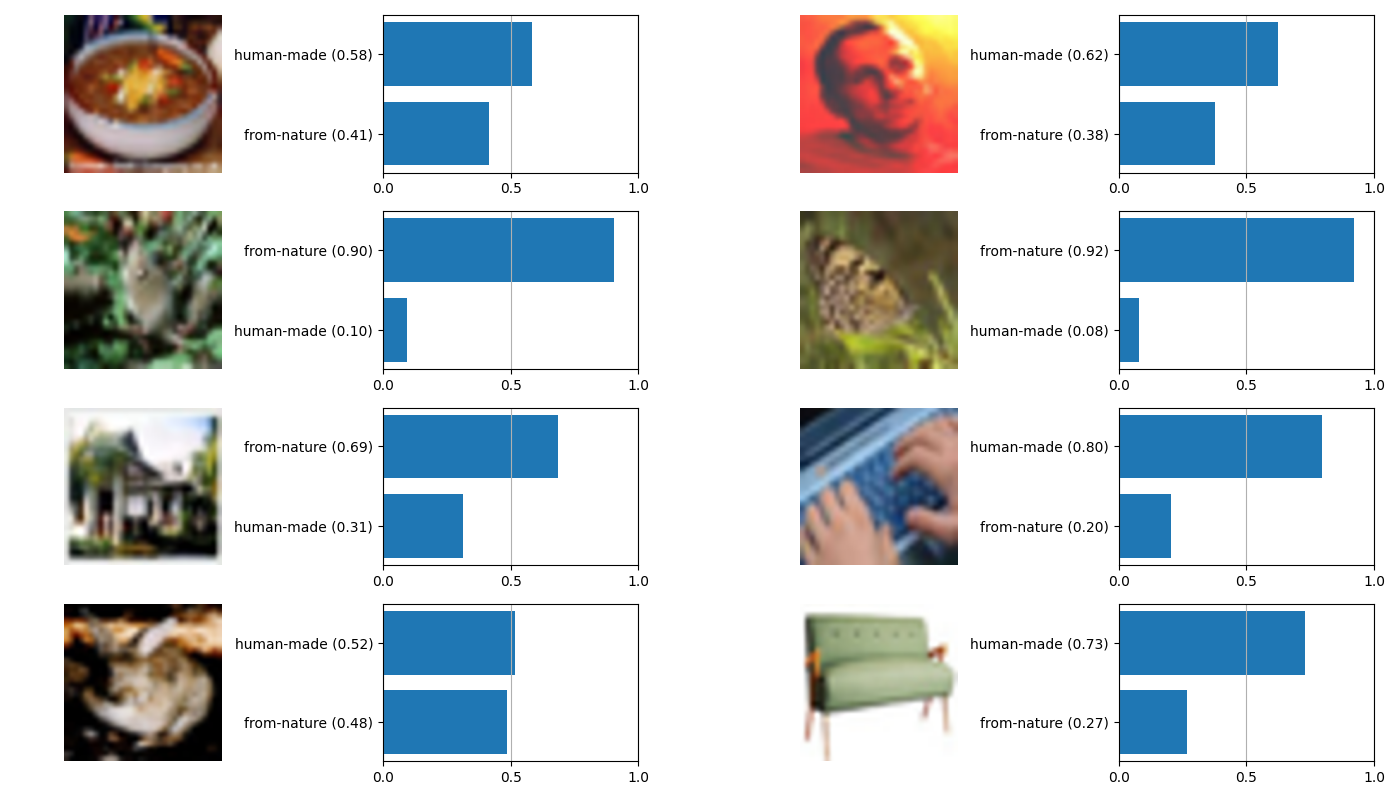
\includegraphics[width=0.75\linewidth]{"imgs/cifar100-test_human-made,from-nature.png"}
    \caption{Distinguishing Human-made and Natural Objects}
    \label{fig:CLIP-human-vs-nature}
\end{figure}

Here too the model performs quite well, considering the task is slightly more abstract than identifying just primary
colours. For clearly human-made objects like a computer keyboard or a couch, the model is able to identify it with
high confidence. It does however mislabel some examples, like the image of the bunny being labelled as human-made. The
more even spread of probabilities for the bunny image suggests that the model is not very confident in its prediction.
See Figure \ref{fig:CLIP-human-vs-nature}.

\bigskip
It therefore seems that CLIP is able to generalize well to new tasks using prompting, but it is not perfect and can
make mistakes when the task is more abstract.
This approach to zero-shot learning is very powerful because it allows us to perform a wide range of tasks without
having to train a new model for each task. This is especially useful when the task is not very complex and does not
require a lot of training data, because training a new model for each task would be very inefficient.
\bigskip

\subsection{Effect of Prompt Types on Classification Accuracy}
\begin{figure}[h]
    \centering
    \begin{minipage}[b]{0.45\linewidth}
        \centering
        
\includegraphics[width=0.8\linewidth]{"imgs/prompt_fixed_patch.png"}
        \caption{Fixed Patch Visual Prompt (Single Pixel Top-Left)}
        \label{fig:prompt-fixed}
    \end{minipage}
    \hfill
    \begin{minipage}[b]{0.45\linewidth}
        \centering
        
\includegraphics[width=0.8\linewidth]{"imgs/prompt_padding.png"}
        \caption{Padding Visual Prompt}
        \label{fig:prompt-padding}
    \end{minipage}
\end{figure}

% CIFAR-10 fixed_patch and prompt size 1 Acc@1 89.570
% CIFAR-10 padding and prompt size 30 Acc@1 92.740
% CIFAR-100 fixed_patch and prompt size 1 Acc@1 64.490
% CIFAR-100 padding and prompt size 30 Acc@1 71.390
\begin{table}[h]
    \centering
    \begin{tabular}{|l|c|c||c|}
    \hline
    \rowcolor{Gray}
    \textbf{Dataset} & \textbf{Fixed Patch Accuracy (\%)} & \textbf{Padding Accuracy (\%)} & \textbf{Baseline Accuracy (\%)} \\ \hline
    CIFAR-10 & 89.57 & 92.74 & 88.94 \\ \hline
    CIFAR-100 & 64.49 & 71.39 & 63.15 \\ \hline
    \end{tabular}
    \caption{CLIP Top-1 Accuracy on CIFAR-10 and CIFAR-100's Test with Different Prompt Types Compared to Baseline}
    \label{tab:clip_accuracy_prompt_types}
\end{table}

Comparing these results obtained using visual prompts on the CIFAR-10 and 100 test set to the baseline results in
seen in Table \ref{tab:clip_accuracy}, we see that the accuracy is higher for both prompt types, with the padding
prompt type performing significantly better than the fixed patch prompt type. This is likely because the padding
prompt type has a lot more trainable parameters (69840 for padding size 30) than the fixed patch prompt type (3 for
patch size 1, one per channel), and thus is able adapt better to the task. Espeically for the CIFAR-100 dataset this
improvement is noticeable. likely due to the fact that the CIFAR-100 dataset is more complex than the CIFAR-10
dataset, and thus requires more trainable parameters to perform well.
\bigskip

\subsection{Deep Prompts}
From Figure 3 in the assignment PDF we see how we can inject a learnable deep prompt into the CLIP model. In the
diagram it is appended to the beginning of the sequence that is fed into a Transformer block. I initially accidentally
appended it to the end of the sequence, but then chose to compare the two approaches which was quite interesting to
see. I also investigated the effect of different numbers of deep prompts (1, 4 \& 8) as well as the injection layer.
The results are shown in Table \ref{tab:clip_accuracy_deep_prompts}, as well as a comparison between the best visual
prompt accuracies and baseline readings in Table \ref{tab:clip_accuracy}.

\begin{table}[h]
    \centering
    \begin{tabular}{|l|c|c|c|c|}
    \hline
    \rowcolor{Gray}
    \textbf{Dataset} & \textbf{Injection Layer} & \textbf{Prompts} & \textbf{Front Acc (\%)} & \textbf{Back Acc (\%)} \\ \hline
    \multirow{9}{*}{CIFAR-10}  
                               & \multirow{3}{*}{0} & 1 & 95.32 & \textbf{95.48} \\ \cline{3-5}
                               &                     & 4 & \textbf{96.31} & 94.97 \\ \cline{3-5}
                               &                     & 8 & \textbf{96.59} & 94.67 \\ \cline{2-5}
                               & \multirow{3}{*}{6} & 1 & 94.63  & \textbf{94.82} \\ \cline{3-5}
                               &                     & 4 & \textbf{95.82} & 94.46 \\ \cline{3-5}
                               &                     & 8 & \textbf{96.00} & 94.23 \\ \cline{2-5}
                               & \multirow{3}{*}{11}& 1 & 91.17  & \textbf{92.44} \\ \cline{3-5}
                               &                     & 4 & 91.18  & \textbf{92.35} \\ \cline{3-5}
                               &                     & 8 & 89.25  & \textbf{92.19} \\ \hline
    \multirow{9}{*}{CIFAR-100} 
                               & \multirow{3}{*}{0} & 1 & 75.90  & \textbf{76.27} \\ \cline{3-5}
                               &                     & 4 & \textbf{78.43} & 75.78 \\ \cline{3-5}
                               &                     & 8 & \textbf{79.98} & 74.86 \\ \cline{2-5}
                               & \multirow{3}{*}{6} & 1 & 73.72  & \textbf{74.29} \\ \cline{3-5}
                               &                     & 4 & \textbf{76.95} & 74.01 \\ \cline{3-5}
                               &                     & 8 & \textbf{78.11} & 73.56 \\ \cline{2-5}
                               & \multirow{3}{*}{11}& 1 & \textbf{69.62} & 68.39 \\ \cline{3-5}
                               &                     & 4 & \textbf{69.61} & 68.00 \\ \cline{3-5}
                               &                     & 8 & \textbf{69.64} & 67.67 \\ \hline
    \end{tabular}
    \caption{Image Classification Performance with CLIP using Different Numbers of Prompts, Injected at Different Layers and Appended to the Front or Back of the Sequence}
    \label{tab:clip_accuracy_deep_prompts}
\end{table}

Injecting prompts at early layers yields higher classification performance across the board than at later layers. This could be because it allows the model to learn more specialized lower-level
features that are more useful for the classification task at hand, although this could differ with dataset too. The
difference between injecting at layer 0 and 6 is also less pronounced than between layer 6 and 11, which might hint to
the fact that deep prompts are most useful for lower-level to mid-level features.
\newline \newline
Increasing the number of prompt generally correlates well with an increase in classification accuracy too, having
the largest effect when injecting at early to middle layers on the CIFAR-100 dataset. This could be because the
CIFAR-100 dataset is more complex than the CIFAR-10 dataset and the model benefits from having more guidance from the
prompts.
\newline \newline
Appending the prompts to the front of the sequence does seem to yield
slightly better results than appending them to the back of the sequence. Although the attention mechanism of the
Transformer should allow the model to learn to attend to the prompts regardless of their position in the sequence,
appending our style of prompt (''This is a photo of a \{\}") perhaps is better suited to being at the beginning,
whereas more of a question or summary style prompt could be better suited to being at the end of the sequence. This
is just specularitory and could be interesting for futher investigation.
\newline \newline
We see that the best performing deep prompt model outperforms the visual prompt model, resulting in a considerable
improvement over the baseline model. 
\begin{table}[h]
    \centering
    \begin{tabular}{|l|c|c|c|}
    \hline
    \rowcolor{Gray}
    \textbf{Dataset} & \textbf{Deep Prompt Acc (\%)} & \textbf{Visual Prompt Acc (\%)} & \textbf{Baseline Acc (\%)} \\ \hline
    CIFAR-10 & 96.59 & 92.74 & 88.94 \\ \hline
    CIFAR-100 & 79.98 & 71.39 & 63.15 \\ \hline
    \end{tabular}
    \caption{CLIP Top-1 Accuracy on CIFAR-10 and CIFAR-100's Test Set with Different Prompt Types Compared to Baseline}
    \label{tab:clip_accuracy}
\end{table}

The reason why deep prompts might outperform the visual prompts is that they can interact with the latent
representation of the image in the model, allowing more complex interactions between the prompt and the image. This
can guide the network better than the visual prompts which only can augment the raw input data.

\subsection{Robustness to Noise}
I investigated how robust CLIP and Resnet-18 are to distributional shifts on CIFAR-100 by adding Gaussian noise to
the test set. The previously trained CLIP model using a visual padding prompt of size 30 on the CIFAR-100 dataset
was used for this, while for Resnet-18 the fine-tunned model was used where only the fully connected layer was
retrained - but not the one being shown augmented data during training as to not bias it towards having seen noisy
data before.

Previously, in this configuration CLIP achieved a test accuracy of 71.39\% and Resnet-18 achieved a test accuracy
of 58.55\%. The results of adding Gaussian noise to the test set are shown in Table \ref{tab:robustness}.

\begin{table}[h]
    \centering
    \begin{tabular}{|l|c|c|}
    \hline
    \rowcolor{Gray}
    \textbf{Test Dataset} & \textbf{CLIP Accuracy (\%)} & \textbf{Resnet-18 Accuracy (\%)} \\ \hline
    CIFAR-100 & 71.39 & 58.55 \\ \hline
    CIFAR-100 + Gaussian Noise & 61.89 & 25.15 \\ \hline
    \end{tabular}
    \caption{CLIP and Resnet-18 Top-1 Accuracy on CIFAR-100's Test Set with and without Gaussian Noise}
    \label{tab:robustness}
\end{table}

Where we can see a clear drop in accuracy for both models, although CLIP seems much more robust to the noise than
Resnet-18, CLIP lost around 10\% accuracy while Resnet-18's more than halved.

The reason this might occur could come down to the learned visual prompts. CLIP's visual prompts perhaps allow it
to learn more robust features that are more invariant to noise, with the padding prompt type of size 30 being able
to attend to a large part of the image and thus being able to learn less sensitive features. Resnet-18 on the other
hand only had its final fully connected layer retrained, which might not help it to be more robust to noise, if
anything it might make it more inclined to overfit to the training data it saw during fine-tuning.
\bigskip

\subsection{Visual Prompts Effectiveness on CIFAR-110}
For investigating the effectiveness of learned visual prompts the best performing visual prompt models, one trained
on CIFAR-10 and one trained on CIFAR-100. When comparing the performance of these on the 110-way classification
task, we see that the model trained on CIFAR-100 performs better than the model trained on CIFAR-10, achieving a
slightly higher test top-1 accuracy (see Table \ref{tab:cifar110}).

\begin{table}[h]
    \centering
    \begin{tabular}{|l|c|c|}
    \hline
    \rowcolor{Gray}
    \textbf{Dataset} & \textbf{CIFAR-10 Prompt Acc (\%)} & \textbf{CIFAR-100 Prompt Acc (\%)} \\ \hline
    CIFAR-110 & 67.705 & 70.525 \\ \hline
    \end{tabular}
    \caption{CLIP Top-1 Accuracy on CIFAR-110's Test Set with Different Prompt Types}
    \label{tab:cifar110}
\end{table}

This is the expected result because the model trained on CIFAR-100 has already seen most of the classes in CIFAR-110,
and thus is able to perform better on it than the model trained on CIFAR-10. The fact that having only seen $<$
10\% of the classes in CIFAR-110 the model trained on CIFAR-10 is able to achieve a test accuracy of 67.705\% is
quite impressive, and shows the power of CLIP's zero-shot learning capabilities and the learned visual prompts.

\subsection{Transfer Learning vs Prompting}
\subsubsection{What are some advantages of prompting over linear probing in terms of robustness against distributional shifts?}
\begin{itemize}
    \item Parameter Optimization Efficiency
    \item Less Compute for Input Manipulation
\end{itemize}

\subsubsection{What are some advantages of prompting over linear probing concerning computational resources?}
\begin{itemize}
    \item Prompt Dataset Overfitting Prevention
\end{itemize}

\subsubsection{What represents some drawback(s) of prompting compared to linear probing concerning memory requirements?}
\begin{itemize}
    \item Increased Memory Load for Prompting
\end{itemize}

\subsubsection{What represents a disadvantage of prompting compared to full fine-tuning and linear probing in terms of adaptability to downstream tasks?}
\begin{itemize}
    \item Limited Data Space Manipulation
\end{itemize}


% ==============================
\section{Graph Neural Networks}
\subsection{Adjacency Matrices}
\subsubsection{}
First graph:\newline
[[0, 1, 1, 1, 1, 1, 1], [1, 0, 0, 0, 0, 0, 0], [1, 0, 0, 0, 0, 0, 0], [1, 0, 0, 0, 0, 0, 0], [1, 0, 0, 0, 0, 0, 0], [1, 0, 0, 0, 0, 0, 0], [1, 0, 0, 0, 0, 0, 0]]\newline\newline
Second graph:\newline
[[0, 1, 1, 1, 1, 1, 1], [1, 0, 1, 0, 0, 0, 1], [1, 1, 0, 1, 0, 0, 0], [1, 0, 1, 0, 1, 0, 0], [1, 0, 0, 1, 0, 1, 0], [1, 0, 0, 0, 1, 0, 1], [1, 1, 0, 0, 0, 1, 0]]\newline\newline
Third graph:\newline
[[0, 1, 0, 0, 0, 1], [1, 0, 1, 0, 0, 0], [0, 1, 0, 1, 0, 0], [0, 0, 1, 0, 1, 0], [0, 0, 0, 1, 0, 1], [1, 0, 0, 0, 1, 0]]

\subsubsection{}
[[2 0 1 0 1 0], [0 2 0 1 0 1], [1 0 2 0 1 0], [0 1 0 2 0 1], [1 0 1 0 2 0], [0 1 0 1 0 2]]

\subsubsection{}
$(A^2)_{uv}$ represents the number of paths of length 2 from node $u$ to node $v$ in the graph. This extends to 
$(A^n)_{uv}$ representing the number of paths of length $n$ from node $u$ to node $v$ in the graph.
\bigskip
% ------------------------------

\subsection{Graph Convolution}
% For an undirected graph with $N$ nodes, each node $v$ is associated with a $d$-dimensional embedding $h_v$. Let us
% consider the following graph convolution that propagtaes the embeddings for all nodes from a layer $l$ to the next
% layer $l+1$:
% $$h_v^{(l+1)} = \sigma \left( W^{(l)} \sum_{u\in N(v)} \frac{h_u^{(l)}}{|N(v)|} + B^{(l)} h_v^{(l)} \right)$$
% The nonlinearity, e.g. ReLU, is denoted by $\sigma$. The matrices
% $B^{(l)}$, $W^{(l)}$ $\in \mathbb{R}^{d^{(l+1)} \times d^{(l)}}$ are parameterizing the self-connection and the
% combination of neighboring node activations respectively. The neighborhood of a node $v$ is denoted by $N(v)$ and
% consists of all nodes connected to $v$ by an edge. Hence, $|N(v)|$ is the number of neighbors of $v$.
\subsubsection{Where in the Equation does the Structural Information on the Graph Appear?}
The structural information on the graph appears in the equation through the term
$$\sum_{u\in N(v)} \frac{h_u^{(l)}}{|N(v)|}$$
This sum represents the aggregation of the embeddings of the neighbours of node v, weighted by the inverse degree of
each neighbour node. This is then multiplied by the weight matrix $W^{(l)}$ to combine the embeddings of the
neighbours into a single embedding for node v after adding the self-connection term $B^{(l)}h_v^{(l)}$ and applying
the nonlinearity $\sigma$.

\subsubsection{How is the graph convolution related to message passing neural networks?}
% In message-parsing neural networks, after every layer, the information contained in the embeddings of a node is
% propagated to the neighbor nodes in so called messages. These are summed up to update the node embedding:
% $$m_v^{(l+1)} = \sum_{u\in N(v)} \text{message}(h_v^{(l)}, h_u^{(l)}, e_{uv})$$
% $$h_v^{(l+1)} = \text{update}(h_v^{(l)}, m_v^{(l+1)})$$
% Here ``message'' and ``update'' are nonlinear functions that can parametrized by artificial neural networks.
A graph convolution can be seen as a subclass of a message passing scheme, where in a graph convolution we are
limited to the immediate neighbours of a node and the message and update functions are parametrized by linear
transformations. In a message passing scheme we can define the message and update functions more flexibly, and we can
propagate messages to nodes that are not immediate neighbours of a node.
\bigskip
% ------------------------------

\subsection{Graph Convolutions Continued}
% The degree matrix $D$ of a graph with $N$ nodes is an $N\times N$ diagonal matrix. For each node $v$, it counts the
% nodes in its neighbourhood $N(v)$:
% $$D_{vu} = \begin{cases}
%     |N(v)| & \text{if } u = v \\
%     0 & \text{else}
% \end{cases}$$

\subsubsection{Rewriting the Graph Convolution in Matrix Form}
% Rewrite the graph convolution to matrix form $H^{(l+1)} = f(H^{(l)})$ with embedding matrix
% $$H^{(l)} = \left[ h_1^{(l)}, \dots, h_{|V|}^{(l)} \right]^T$$
% Use the adjacency matrix $A$ and the degree matrix $D$.
Using the Adjacency matrix $A$ and the Degree matrix $D$, we can rewrite the graph convolution to matrix form as
follows:
$$H^{(l+1)} = \sigma \left( W^{(l)} D^{-1} A H^{(l)} + B^{(l)} H^{(l)} \right)$$
Where $D^{-1}AH^{(l)}$ represents the normalized sum of the embeddings of the neighbours. 

\subsubsection{Which function does this graph convolutional network use to aggregate over neighboring nodes?}
The graph convolutional network uses the mean function to aggregate over neighbouring nodes. Its the sum of all
neighbouring embeddings divided by the number of neighbours.

\subsubsection{Is Rewriting to Matrix Form Possible for All Aggregation Functions?}
No, rewriting to matrix form is not possible for all aggregation functions. The aggregation function must be
applicable uniformly across all nodes and their neighbours. Max pooling for example is not applicable because it
would require a different number of neighbours for each node, and thus a different number of terms in the sum for each
node. This coupled with its nonlinearity makes it impossible to rewrite to matrix form.

\bigskip
% ------------------------------

\subsection{Connections to Standard Neural Network Architectures}
% In principle, we can concatenate the adjacency matrix and node embeddings to classify each data point with a
% standard feed-forward neural network. What problems do you expect with this approach? Where does it fail completely?
% Name three different aspects. Keep in mind different applications: for example, classifiying molecular structures
% in chemistry (i.e. graph classification) or categorizing people in a social network (i.e. node classification).
% Being concise and to the point will help you get all the points.
Firstly, scaling to larger graphs would be difficult because the adjacency matrix would grow quadratically with the
number of nodes in the graph. This would make the input to the feed-forward neural network very large and thus
computationally expensive to train and evaluate. For social networks for example with millions of people, this would
be infeasible.
\newline \newline
Secondly, the loss of structural information would be problematic. The adjacency matrix would be flattened and
concatenated with the node embeddings, and thus the structural information would be lost. This would make it
difficult to learn from the graph structure, which is the main advantage of graph neural networks. For example, in
chemistry the structure of the molecule is very important for its properties, and thus this approach would not be
suitable.
\newline \newline
Thirdly, the approach lacks invariance to node permutations. The same graph can be represented by multiple adjacency
matrices, depending on the ordering of nodes. When concatenating a flattened adjacency matrix with
node embeddings, different permutations of the same graph would result in different input vectors to the feed-forward
neural network. This lack of permutation invariance of a FFNN could lead to inconsistent model performance, as the
network might interpret these permutations as distinct graphs. This could be an issue in for example molecular
structure classification, where different representations of the same graph should yield the different predictions.
\bigskip
% ------------------------------
\subsection{Relation to Transformers}
\subsubsection{How can a Transformer Model be Seen as a Graph Neural Network?}
% Consider a standard transformer model applied to a sentence in natural language. How can a transformer model be seen
% as a graph neural network? What would be the nodes and edges, and what would be the graph structure?
The nodes in this case would be the words in the sentence, and the edges would be the attention weights between
the nodes. The graph structure would be a fully connected graph, where each node is connected to every other node,
and the attention scores between words represent the edge weights.

\subsubsection{How Can the Transformer Model Process Inputs for Which the Order Matters While Staying Permutation
Invariant in its Architecture and Computation?}
% Transformers perform state-of-the-art in the natural language domain, which is inherently not permutation invariant:
% it matters in which order we say something. How can the transformer model process inputs for which the order matters
% while staying permuation invariant in its architecture and computation?
Transformers encode the order of the input sequence in positional embeddings, which are added to the input embeddings
before being fed into en/decoder. This allows the model to retain information and learn from the order of the input
sequence. The self-attention mechanism which is used to compute the attention scores is permutation invariant, and
thus the model is permutation invariant in its architecture and computation.

\end{document}